\documentclass[final,xcolor=dvipsnames]{beamer}
%
% Choose how your presentation looks.
%
% For more themes, color themes and font themes, see: 
% http://deic.uab.es/~iblanes/beamer_gallery/index_by_theme.html
%
\mode<presentation>
{
  \usetheme{Boadilla}      % or try Darmstadt, Madrid, Warsaw, ...
  \usecolortheme{default} % or try albatross, beaver, crane, ...
  \usefonttheme{structurebold}  % or try serif, structurebold, ...
  \setbeamertemplate{navigation symbols}{}
  \setbeamertemplate{caption}[numbered]
} 

\usepackage[english]{babel}
\usepackage[utf8x]{inputenc}
\usepackage[]{caption}
\usepackage{tikz}



%the-sun-is-in-love-with-the-moon-collab-with-blaak.jpg

%\titlegraphic{
\includegraphics[]{the-sun-is-in-love-with-the-moon-collab-with-blaak.jpg} \hspace{2cm} \includegraphics[width=2cm]}}
\title[Resource Competition]{Resource Competition and Community Structure}
\subtitle{OCEA0096-1 	Modélisation des écosystèmes et des cycles biogéochimiques : Partim Ressources}
\author[A. Capet]{A. Capet - acapet@ulg.ac.be} %Logo de MAST +logo interface sur chaque slide et page de garde interface?
\institute[http://labos.ulg.ac.be/mast/]{MAST}
\date[2017-2018]


\AtBeginSection[]{
  \begin{frame}
  \vfill
  \centering
  \begin{beamercolorbox}[sep=8pt,center,shadow=true,rounded=true]{title}
    \usebeamerfont{title}\insertsectionhead\par%
  \end{beamercolorbox}
  \vfill
  \end{frame}
}

\begin{document}

% \usebackgroundtemplate{%             declare it
% \tikz[overlay,remember picture] \node[opacity=0.6, at=(current page.center)] {
%   
\includegraphics[height=\paperheight,width=\paperwidth]{the-sun-is-in-love-with-the-moon-collab-with-blaak.jpg}
%   };
%   % {Great_Barrier_Reef_Australia}};
% }

\begin{frame}
  \titlepage
\end{frame}


% \usebackgroundtemplate{ }  

\section{Basics}

\begin{frame}{What are ressources ?}
 A factor that
 \begin{itemize}
 \item has a given availability
 \item leads to higher growth as availability increases
 \item is consumed by the population(s)
 \end{itemize}
 Multiple factors can be considered as resources if they meet the above criteria for some range of other factors availability.
\end{frame}

\begin{frame}{Consumption for Growth model}
For $n$ species competing for $k$ resources :
  \begin{eqnarray}
  \frac{d~N_i}{N_i~dt}&=&f_i(R_1,...,R_k) - m_i \\
  \frac{d~R_j}{dt}&=&g_j(R_j)-\sum\limits_{i=1}^n N_i f_i(R_1,...,R_k) h_{i,j}(R_1,...,R_k)
  \end{eqnarray}
  \begin{tabular}{c p{10cm}}
  $N_i$ & population density of species $i$\\
  $R_j$ & availability of resource $j$ \\
  $f_i$ & functional relationship between $R_j$ and rate of population changes for $N_i$ \\
  $g_j$ & resource supply \\
  $m_i$ & mortality rate for species $i$ \\
  $h_{i,j}$ & amount of resource $j$ required to create a new individual $i$
  \end{tabular}
\end{frame}


\begin{frame}{Assumptions}
\begin{itemize}
\item pure competition : $\frac{\partial f_i}{\partial N_j}=0$
\item resources are not interactives : $\frac{\partial g_i}{\partial R_j}=0$ for $i\neq j$
\end{itemize}
\end{frame}

\section{One resource}

\begin{frame}{One resource}
\begin{figure}
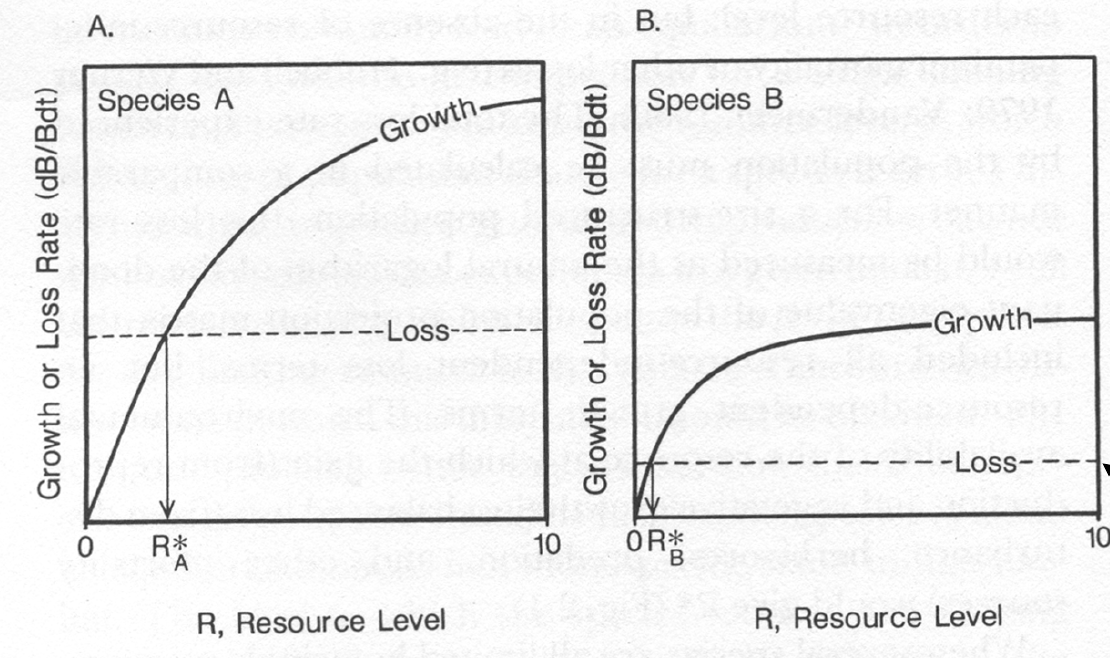
\includegraphics[width=.5\framewidth]{1ressourceGrowth}
\includegraphics<2>[width=.4\framewidth]{1RessourceCompetition}
\end{figure}
\only<1>{
\begin{eqnarray}
  \frac{1}{N}\frac{\partial~N}{\partial t}&=&f(R) - m \\
   f(R*) & =&  m \Rightarrow \frac{\partial~N}{N~\partial t} =0 
   \end{eqnarray}}
\begin{block}<1->{$R^*$}
The resource level for which growth = mortality.
\end{block}
\begin{block}<2>{The $R^*$ Theory}
If only one resource, the species with the lower R* overcompetes the others. 
\end{block}
\end{frame}

\section{Two resource}

\begin{frame}{Growth Isoclines}
In the "resource-space", the $\gamma$-growth isoline is the locus $f_i(R_1,R_2)=\gamma$
\begin{figure}
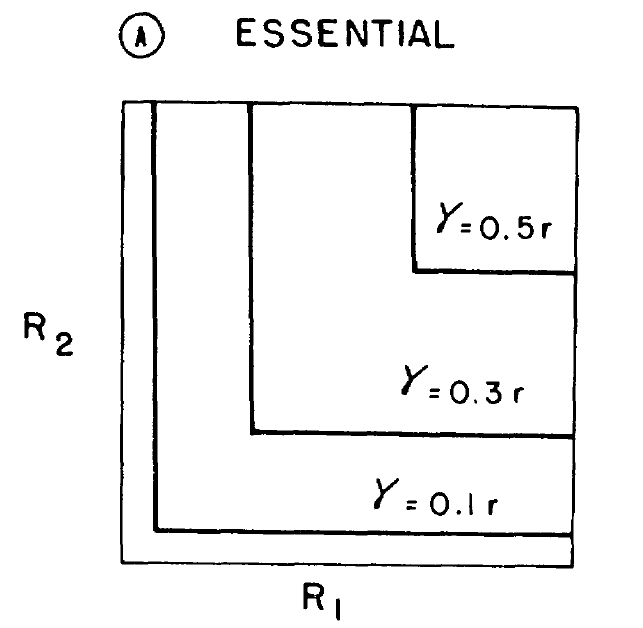
\includegraphics[width=.4\framewidth]{Essential1}
\end{figure}
Different shape for different type of resources\\
Note that $\gamma$ is the reproduction rate without mortality.
\end{frame}

\section{Type of resources}

\subsection{Essential Resources}
\begin{frame}[allowframebreaks]{Essential Resources}

     \begin{figure}
       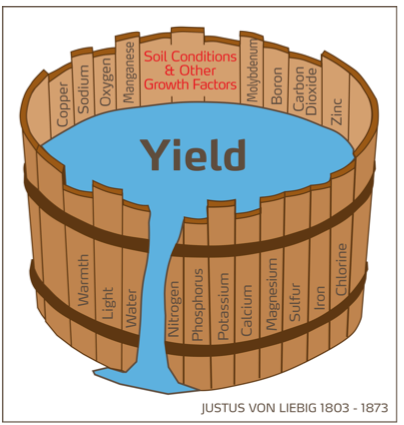
\includegraphics[width=.3\framewidth]{Barrel}
    \end{figure}
Justus von Liebig's law of the minimum, 1873 : \textit{\small If one growth factor/nutrient is deficient, plant growth is limited, even if all other vital factor/nutrient are adequate .. plant growth is improved by increasing the supply of the deficient factor/nutrient.} 	
    \begin{equation}
f(R_1,...,R_k)=\min\limits_{j=1,k} (f_j(R_j))     
    \end{equation}
    
\framebreak

\begin{columns}
  \begin{column}{.6\framewidth}
   \begin{itemize}
   \item No growth possible if one resource is lacking
   \item $f_i(R_1=0,R_2)\leq 0$ for all $R_2$ and $f_i(R_1,R_2=0)\leq 0$ for all $R_1$
   \item iso-growth lines never intersect the axis
   \item Examples
   \begin{itemize}
   \item Nitrate, Phosphate, Light
    \end{itemize}
   \item Counter-Example : $[\mathrm{NO_3^{-}}]$ and $[\mathrm{NO_2^{2-}}]$
   \end{itemize}
  \end{column}
  \begin{column}{.4\framewidth}
    \begin{figure}
       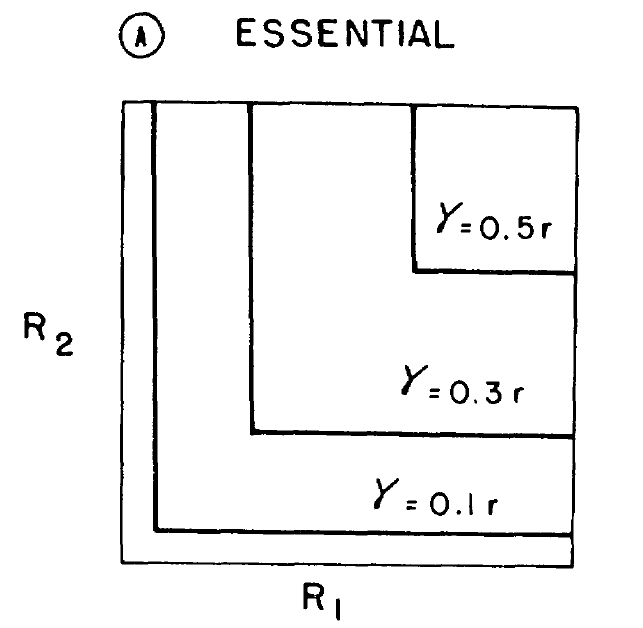
\includegraphics[width=.4\framewidth]{Essential1}
    \end{figure}
  \end{column}
 \end{columns}

 \framebreak


 \begin{columns}
  \begin{column}{.5\framewidth}
  \begin{figure}
       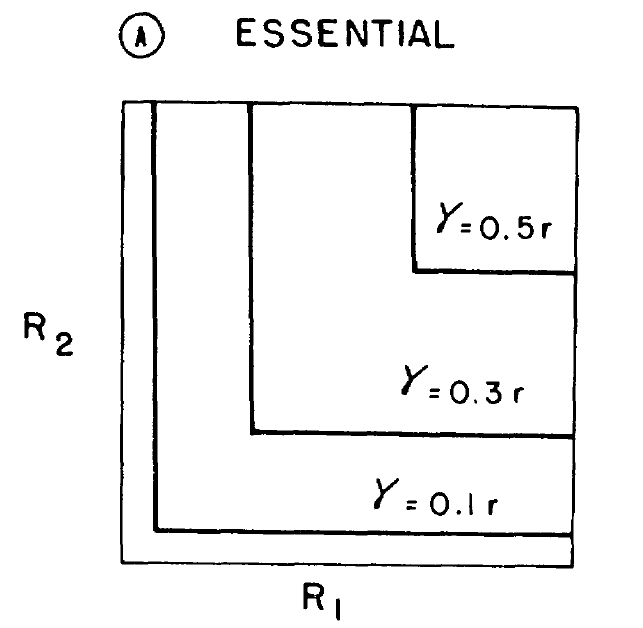
\includegraphics[width=.4\framewidth]{Essential1}
       \caption[]{Noninteractive Essential}
    \end{figure}
  \end{column}
  \begin{column}{.5\framewidth}
    \begin{figure}
       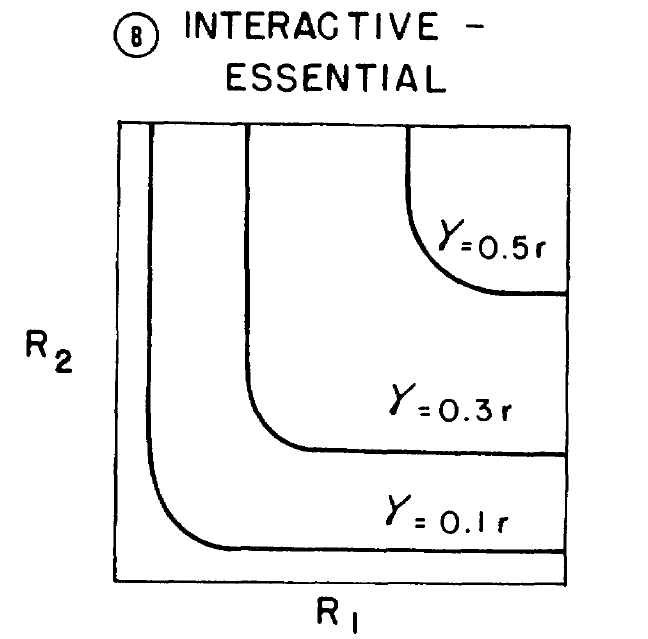
\includegraphics[width=.4\framewidth]{InteractiveEssential1}
              \caption[]{Interactive Essential}
    \end{figure}
  \end{column}
 \end{columns}
 \framebreak

\end{frame}


\begin{frame}{Substitutable Resources}
  \begin{columns}
  \begin{column}{.6\framewidth}
   \begin{itemize}
   \item Any resources can support growth on its own 
   \item $f_i(R_1=0,R_2)> 0$ for some $R_2$ and $f_i(R_1,R_2=0)> 0$ for some $R_1$
   \item iso-growth lines intersect the axis
   \item Examples
   \begin{itemize}
   \item Herbivorous and carnivorous diet
   \end{itemize}
   \end{itemize}
  \end{column}
  \begin{column}{.4\framewidth}
    \begin{figure}
       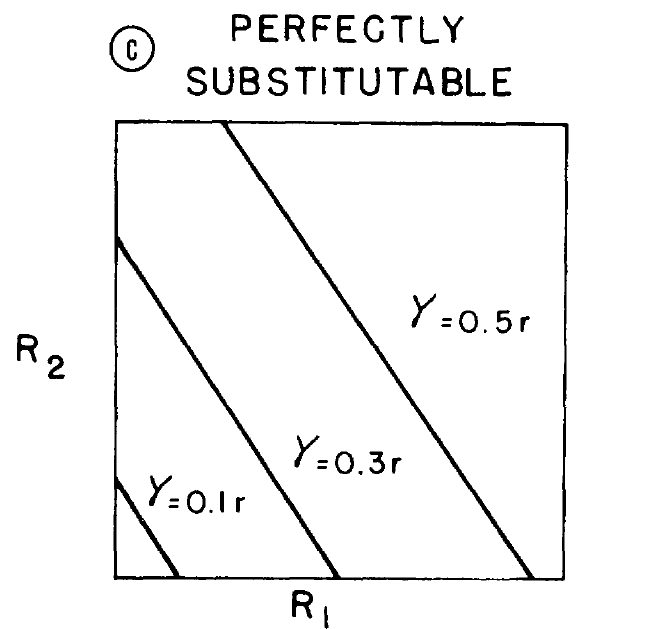
\includegraphics[width=.4\framewidth]{PerfectlySubst1}
    \end{figure}
  \end{column}
 \end{columns}
\end{frame}

\begin{frame}{Substitutable Resources}
 \begin{columns}
  \begin{column}{.33\framewidth}
  \begin{figure}
       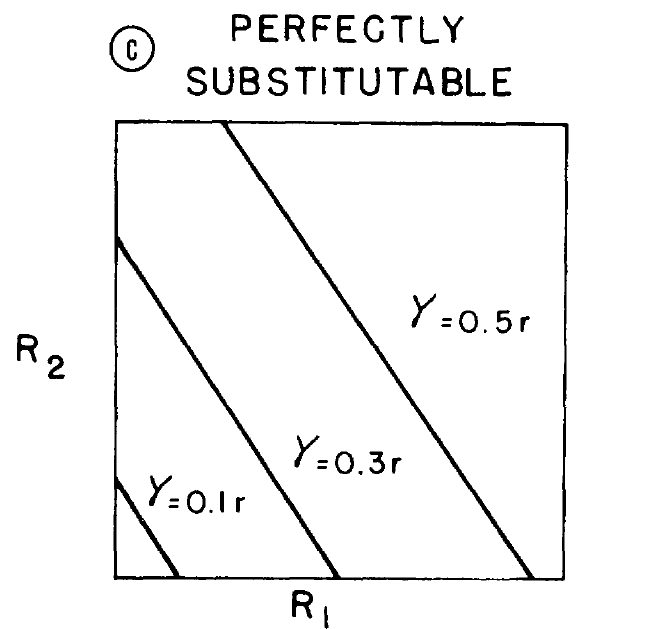
\includegraphics[width=.4\framewidth]{PerfectlySubst1}
      % \caption[]{Perfectly Substitutable}
    \end{figure}
  \end{column}
  \begin{column}{.33\framewidth}
    \begin{figure}
       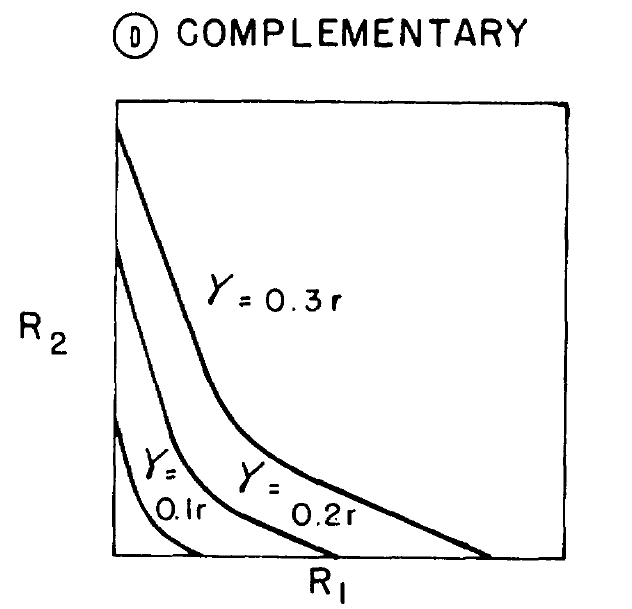
\includegraphics[width=.4\framewidth]{Complementary1}
      %        \caption[]{Interactive Essential}
    \end{figure}
  \end{column}
    \begin{column}{.33\framewidth}
    \begin{figure}
       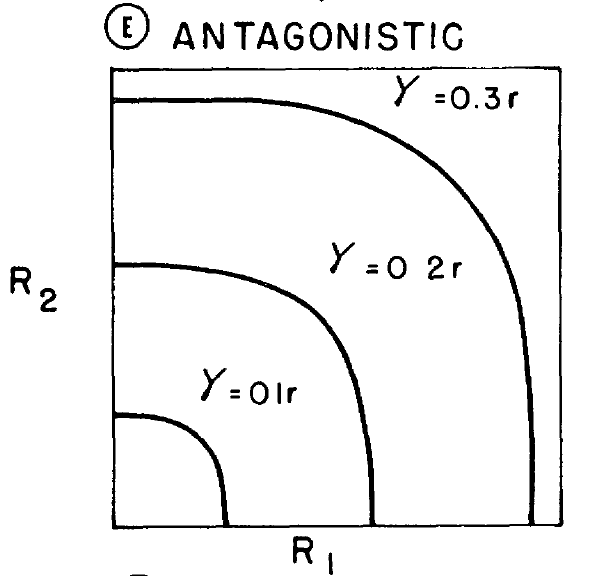
\includegraphics[width=.4\framewidth]{Antagonistic1}
           %   \caption[]{Interactive Essential}
    \end{figure}
  \end{column}
 \end{columns}
\end{frame}

\begin{frame}{Hemi-essential Resources}
  \begin{columns}
  \begin{column}{.6\framewidth}
   \begin{itemize}
   \item One is essential and can support growth on its own , the other can only partly substitute
   \item $f_i(R_1=0,R_2)> 0$ for some $R_2$ and $f_i(R_1,R_2=0)\leq 0$ for all $R_1$
   \item iso-growth lines intersect one axis
   \end{itemize}
  \end{column}
  \begin{column}{.4\framewidth}
    \begin{figure}
       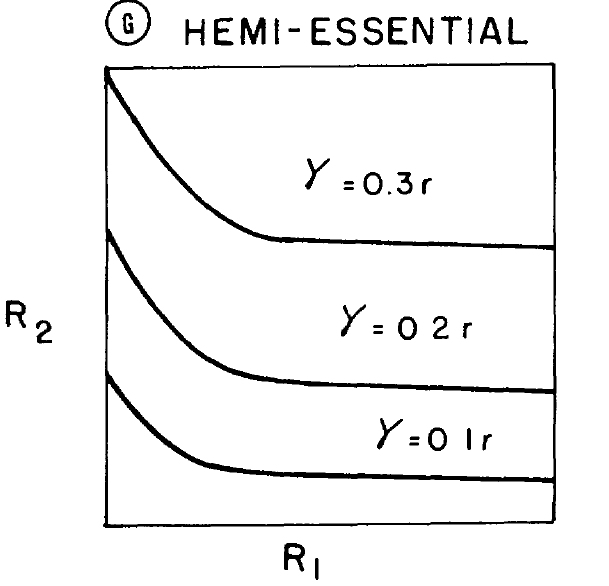
\includegraphics[width=.4\framewidth]{HemiEssentialA1}
    \end{figure}
  \end{column}
 \end{columns}
\end{frame}

%TODO detail consumption vectors with examples

\section{Dynamics}

\begin{frame}{Consumption vectors}  
\only<1>{
\begin{itemize}
\item Represents changes in ressources following consumption for growth
\item Depends on 
\begin{itemize}
\item Consumption(s) per individuals ($\rightarrow$ Characterisitc to species)
\item Number of individuals
\end{itemize}
\end{itemize}
\begin{figure}
       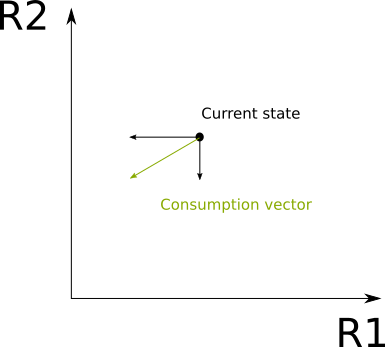
\includegraphics[width=.5\framewidth]{Til1}
    \end{figure}
}
\only<2>{
	\begin{figure}
       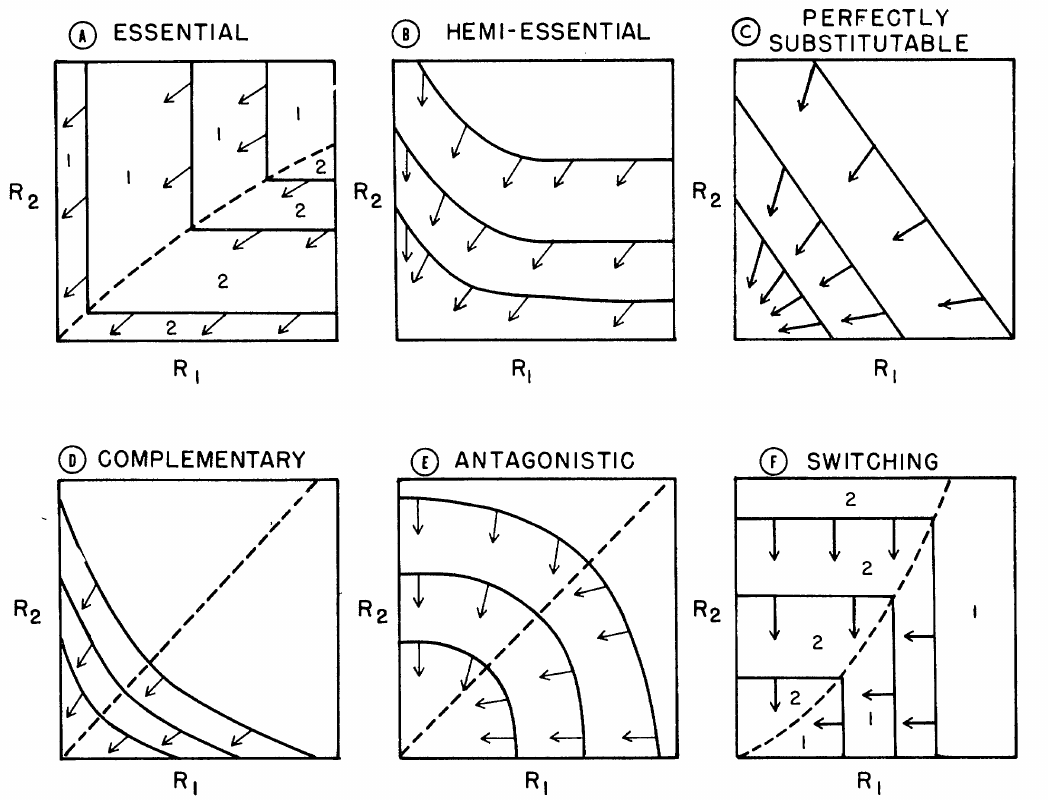
\includegraphics[width=.8\framewidth]{ConsumptionVectors}
    \end{figure}
}
\end{frame}

\begin{frame}{Supply vectors}  
\only<1>{
\begin{itemize}
\item Represents the environmental supply of ressources
\item Depends on 
\begin{itemize}
\item The environment (Supply point)
\item The actual state of resources
\end{itemize}
\end{itemize}
\begin{figure}
       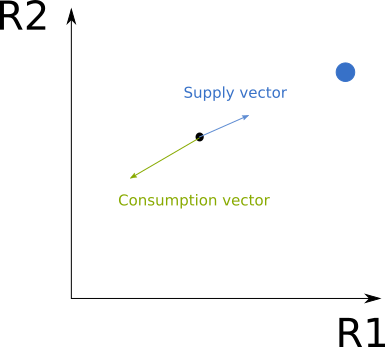
\includegraphics[width=.5\framewidth]{Til2}
    \end{figure}
}
\only<2>{
	\begin{figure}
       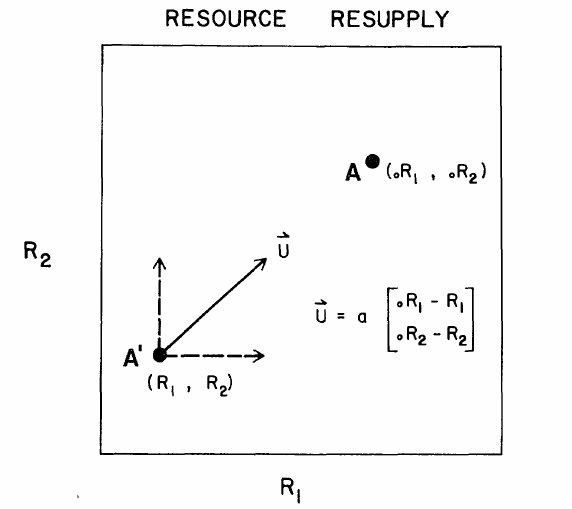
\includegraphics[width=.5\framewidth]{RessourceSupply}
    \end{figure}

   \begin{itemize}
   \item Constant "string" toward supply point
   \item $\frac{d\,R_1}{dt}|_{supply}= a(R_{1,0}-R_1)$ \& $\frac{d\,R_2}{dt}|_{supply}= a(R_{2,0}-R_2)$
%   \item Supply vector $\vec{U} = [ ] $ 
   \end{itemize}
}
\end{frame}

\begin{frame}{One species, two resources}  
\begin{figure}
       \includegraphics<1>[width=.5\framewidth]{ZNGIss}
       \includegraphics<2>[width=.5\framewidth]{Eq} 
   \end{figure} 
\begin{block}<1>{ZNGI}
Zero Net Growth Isoline: where $\gamma$= mortality
\end{block}
\end{frame}

\begin{frame}{Equilibrium point: One species, two resources}  
	\begin{figure}
       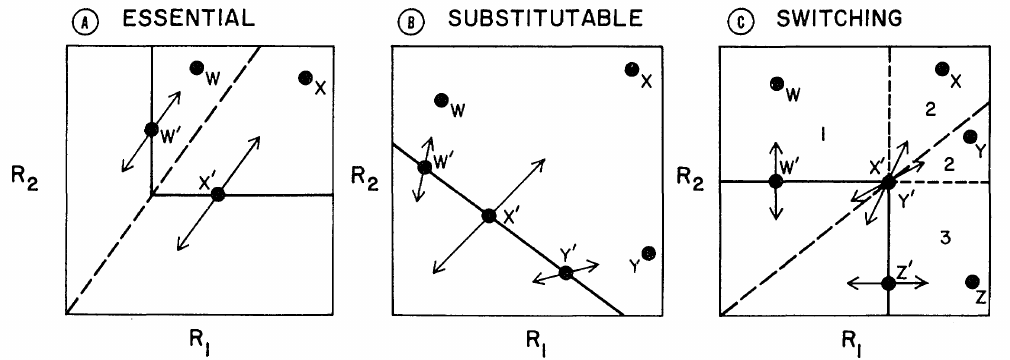
\includegraphics[width=.8\framewidth]{ZNGI}
    \end{figure}
    Equilibrium points set by 
  \begin{itemize}
  \item Consumption vectors
  \item Supply point
  \item ZNGI
  \end{itemize}
\end{frame}


\begin{frame}{Equilibrium Points}  
Examples in R with TILMAN1
\begin{itemize}
\item Present the program
\item iso-growth
\item Consumption vectors
\item Supply Vectors
\item Equilibrium points (show that supply below ZNGI prohibits survival)
\end{itemize}
\end{frame}

%%%%%%%%%%%%%%%%%%
%%    BREAK ? 
%%%%%%%%%%%%%%%%%%

\section{Competition}


\begin{frame}{2 Species : competition}  
  \begin{figure}
    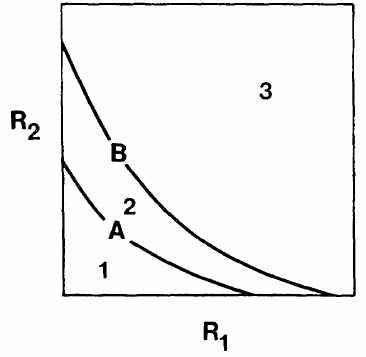
\includegraphics[width=.5\framewidth]{CompQuestion}
  \end{figure}
  \only<1>{\begin{alertblock}{Question}
	What's the outcome of supply point in 1, 2, 3  ?
  \end{alertblock}
  }
  \only<2>{
      \begin{description}
		\item[1] Neither species able to survive
		\item[2] Only A can survive
		\item[3] A removes B by competion
	  \end{description}
	}
  \begin{alertblock}<3>{Question}
    Which condition for coexistence ? 
  \end{alertblock}
\end{frame}

\begin{frame}{2 Species : competition}  
\begin{figure}
       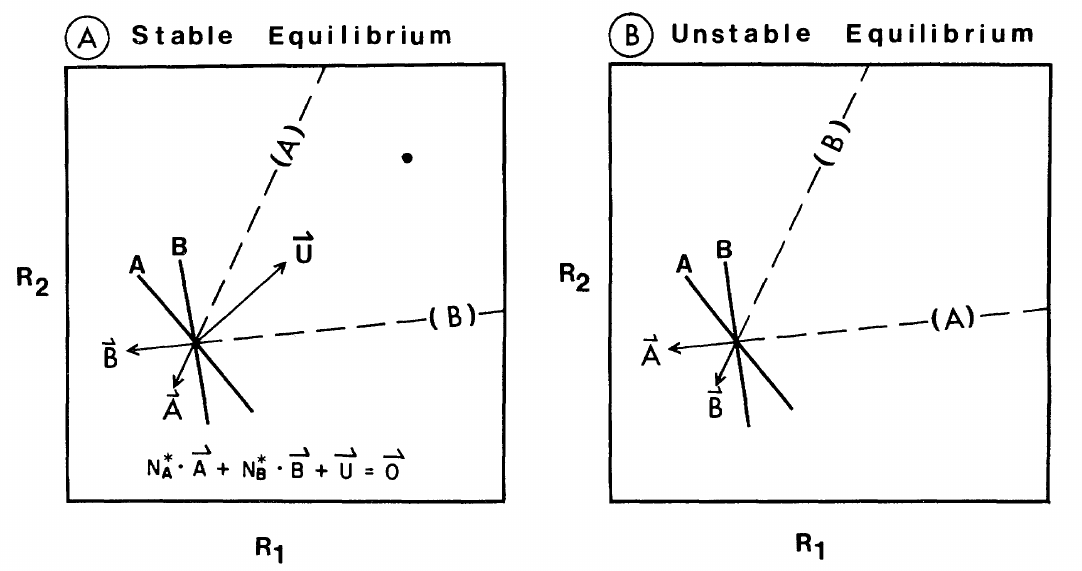
\includegraphics[width=.8\framewidth]{Eq1}
 \end{figure}
\only<1>{
\begin{itemize}
\item Crossings of the ZNGI defines cohabitation equilibrium point
\item Might be stable or unstable 
\end{itemize}
}
\only<2>{
  \begin{block}{Trade-offs}
In resource poor environments, organisms allocate resource for efficiency on one resource $\rightarrow$ less efficiency regarding other resources. \\
Example : Leaves or roots ? 
  \end{block}
}
\only<3>{
Stable if 
 \begin{enumerate}
\item Each species consumes proportionately more of the resources that limits its own growth
\item The amounts of resource consumed by individual changes only slightly in response to small changes in $R_j$
\end{enumerate}
}
\end{frame}

\begin{frame}{2 Species : competition}  
\begin{figure}
       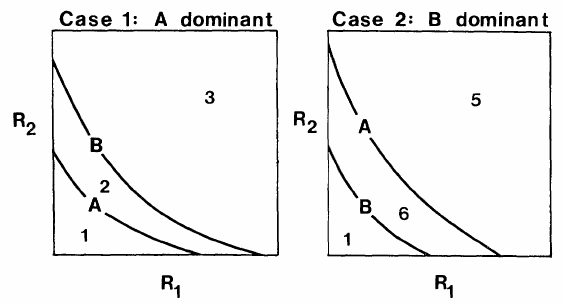
\includegraphics[width=.5\framewidth]{NoCohabitation.png}
       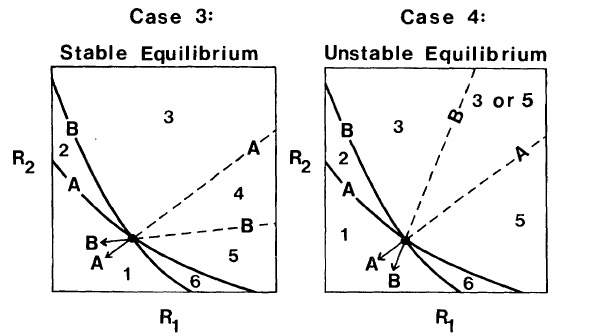
\includegraphics[width=.5\framewidth]{Cohabitation.png}
    \end{figure}
    \begin{columns}
             \begin{column}{.5\framewidth}
              \begin{description}
\item[1] Neither species able to survive
\item[2] Only A can survive
\item[3] A removes B by competition
\end{description}
    \end{column}
        \begin{column}{.5\framewidth}
                          \begin{description}
\item[4] Coexistence
\item[5] B removes A by competition
\item[6] Only A can survive
\end{description}
    \end{column}
    \end{columns}
\end{frame}

\begin{frame}{2 Species : competition}  
\begin{figure}
       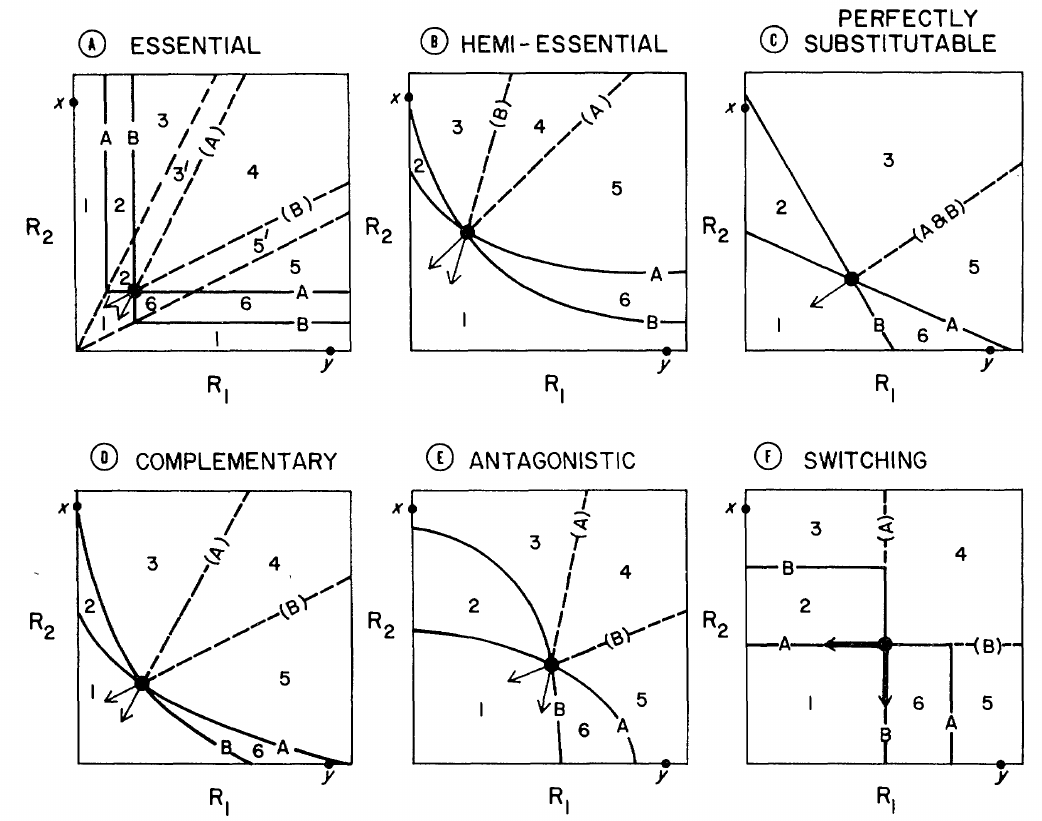
\includegraphics[width=.8\framewidth]{Eq6types}
    \end{figure}
\end{frame}

\begin{frame}{Resource spatial gradients}
\begin{figure}
       \includegraphics<1>[width=.8\framewidth]{Eq6typesB}
       \includegraphics<2>[width=.8\framewidth]{RessourceGradients1}
    \end{figure}
\end{frame}

\begin{frame}{Mixed Resource types}
\begin{figure}
       \includegraphics<1>[width=.6\framewidth]{Mixed1}
       \includegraphics<2>[width=.6\framewidth]{RessourceGradients2}
    \end{figure}
\end{frame}


\begin{frame}{Multi Species}
\begin{figure}
       \includegraphics<1>[width=.6\framewidth]{5Species}
       \includegraphics<2>[width=.6\framewidth]{RessourceGradients3}
       \includegraphics<3>[width=.5\framewidth]{5Species}
    \end{figure}
    \begin{block}<3>{Heterogeneity}
    Variations in resource RATIOS supports species variety
    \end{block}
\end{frame}

\section{Experiments}

\begin{frame}
\begin{figure}
       \includegraphics<1>[width=.8\framewidth]{MillerCitation}
       \includegraphics<2>[width=.45\framewidth]{Miller1}
        \includegraphics<2>[width=.45\framewidth]{Miller2}
\end{figure}
\end{frame}

\begin{frame}{Experiments}
\begin{figure}
       \includegraphics<1>[width=.6\framewidth]{TilTest1}
       \includegraphics<2>[width=.8\framewidth]{TilTest0}
       \includegraphics<3>[width=.8\framewidth]{TilTest3}
    \end{figure}
\end{frame}

\begin{frame}{Experiments}
\begin{figure}
       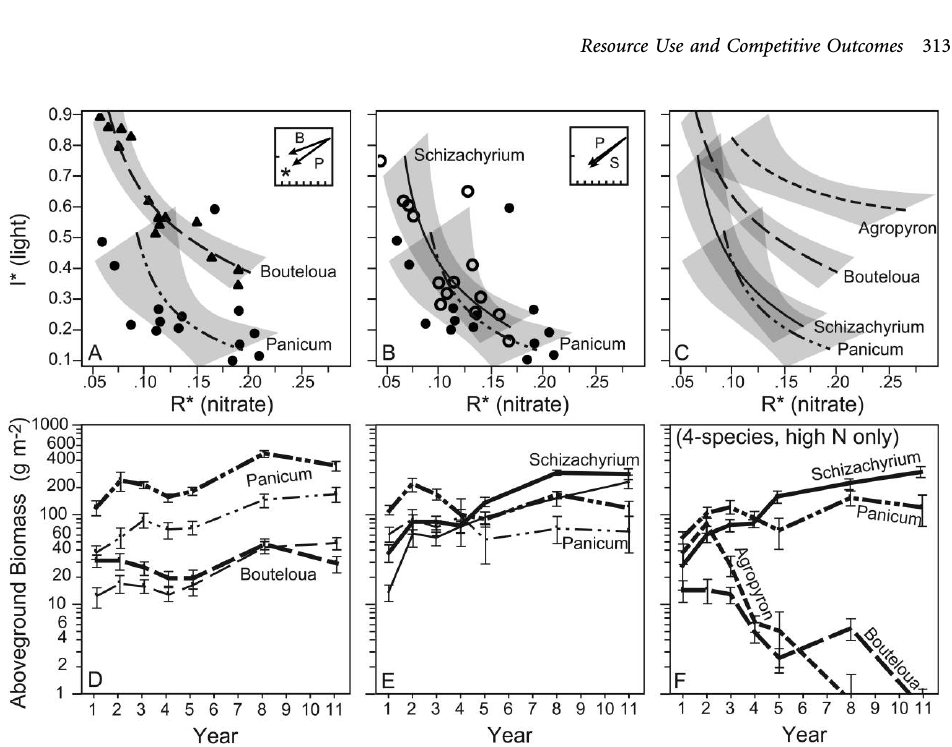
\includegraphics[width=.8\framewidth]{RealCase1}
       \caption{Ray Dybzinski and David Tilman, 2007,\textit{ The American Naturalist}
}
    \end{figure}
\end{frame}


\section{Propositions of investigations}
\begin{frame}
\begin{itemize}
\item Extend R framework for two species, illustrate cases, Monte Carlo to visualize coexistence. 
\item Mixotrophy/Allelopathy
\item Heterogeneity 
\item Investigate Plankton dominance in BS model outputs
\item Fit and identify growth parameters for various species.
\end{itemize}
\end{frame}

\begin{frame}
\begin{figure}
       
\includegraphics[width=.6\framewidth]{TilmanPaperCitation}
    \end{figure}
\end{frame}

\begin{frame}
Recent application : 
\url{http://www.biogeosciences.net/14/2877/2017/}
\end{frame}

\end{document}
